\documentclass{article}
\usepackage[utf8]{inputenc}
\usepackage{graphicx}
\usepackage{listings}
\title{Information System - Lab work 4}
\author{Tran Thi Hong Hanh}
\date{9 November 2017}

\begin{document}

\maketitle
\section*{Database}
\begin{itemize}
	\item employees (emp\_no, birth\_date, first\_name, last\_name, gender)
	\item departments (dept\_no, dept\_name)
	\item dept\_emp (emp\_no, dept\_no, from\_date, to\_date)
	\item dept\_manager (dept\_no, emp\_no, from\_date, to\_date)
	\item titles (emp\_no, title, from\_date, to\_date)
	\item salaries (emp\_no, salary, from\_date, to\_date)
\end{itemize}

\section*{Requirements}
\begin{enumerate}
	\item Update Development (d005) and Research (d008) into Research and Development (d010).
	\item Update Marketing (d001) and Sales (d007) into Marketing and Sales (d011).	
\end{enumerate}

\section*{Main steps \& Explanation}
\begin{enumerate}
	\item Insert new values into "departments". 
	\begin{lstlisting}{showstringspaces=false}[language=SQL]
INSERT INTO departments VALUES
("d010", "Research and Development"),
("d011", "Marketing and Sales");
	\end{lstlisting}
	First and foremost, it's necessary that we add the new information of departments (Research and
Development(d010) and Marketing and Sales (d011)) to avoid the data conflict in schema.

	\item Update information of all employees/managers from original department to new one.\\
	\begin{itemize}
		\item Update dept\_manager:
		\begin{lstlisting}{showstringspaces=false}[language=SQL]
UPDATE IGNORE dept_manager
SET dept_no = 'd010'
WHERE dept_no IN ('d005', 'd008') ;
	
UPDATE IGNORE dept_manager
SET dept_no = 'd011'
WHERE dept_no IN ('d001','d007') ;
	\end{lstlisting}
		\item Update dept\_emp:
		\begin{lstlisting}{showstringspaces=false}[language=SQL]
UPDATE IGNORE dept_emp
SET dept_no = 'd010'
WHERE dept_no IN ('d005', 'd008') ;
	
UPDATE IGNORE dept_emp
SET dept_no = 'd011'
WHERE dept_no IN ('d001','d007') ;
	\end{lstlisting}
	
After the addition of new information to database, the old information (Development (d005) and Research (d008), Marketing (d001) and Sales (d007)) should be updated to the required ones for both dept\_manager and dept\_emp. Thanks to step 1, the tuples can be updated the new value using queries without conflict. 

	\end{itemize}
	\item Delete the old unnecessary information.
	\begin{lstlisting}{showstringspaces=false}[language=SQL]
DELETE FROM departments 
WHERE dept_no IN ('d005', 'd008','d001','d007');
	\end{lstlisting}

\end{enumerate}


\section*{Results}

The result of the process below illustrates in Figure 1 as below:\\
\begin{figure}[h]
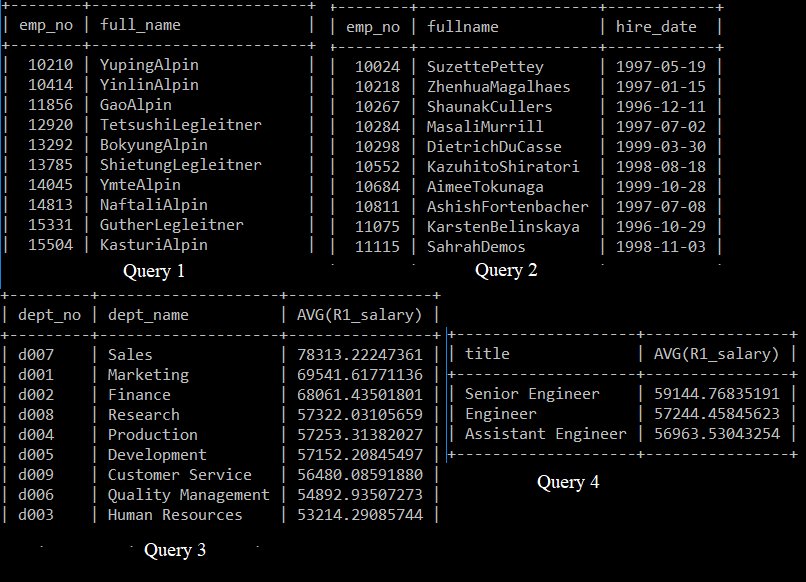
\includegraphics[scale = 0.65]{result.PNG}
\caption{Implementation and results}
\end{figure}

\end{document}
